\setcounter{page}{1}
\section{引言}
\setcounter{figure}{0}
\setcounter{table}{0}

\subsection{模板介绍}

这是一个根据《西南财经大学本科生毕业论文(设计)撰写与印制规范》开发的 \LaTeX 论文模板,适用于Overleaf平台\footnote{\url{https://cn.overleaf.com/}},作者为\textbf{小嗷犬}\footnote{\url{https://marquis.eu.org/}}。模板采用Creative Commons CC BY 4.0协议\footnote{\url{https://creativecommons.org/licenses/by/4.0/legalcode.zh-hans}}开源至GitHub\footnote{\url{https://github.com/Marquis03/SWUFE-Thesis}}。如果该模板对您有所帮助,请在GitHub上帮我点一个小小的Star;如果遇到使用上的问题,欢迎通过电子邮箱与我取得联系\footnote{\href{mailto:marquis128@foxmail.com}{marquis128@foxmail.com}}。

新增内容建议在 \textcolor{cyan}{/content/正文/} 路径下新建 \textcolor{cyan}{.tex} 文件,并按照以下代码模板撰写内容:

\begin{lstlisting}[language=Tex]
\section{你的章节名称}
\setcounter{figure}{0}
\setcounter{table}{0}

%% 你的章节内容
\end{lstlisting}

然后在 \textcolor{cyan}{main.tex} 文件中使用 \textcolor{cyan}{\textbackslash include} 引入该文件。


\subsection{学校概况}

\subsubsection{学校简介}

西南财经大学是教育部直属的国家“211工程”和“985工程”优势学科创新平台建设的全国重点大学,也是国家首批“双一流”建设高校。学校坐落于中国历史文化名城——“天府之国”成都,有光华、柳林两校区,辖地2300余亩。校园湖光柳影,芳草绿树,翩翩学者,蔚为大观,是著名的“园林式院校”,实乃读书治学的理想园地。

学校始于1925年在上海创建的光华大学。1938年,因抗战内迁建立光华大学成都分部。1952-1953年,先后汇聚西南地区17所院校的财经系科组建成四川财经学院,是建国之初全国高等院校分区布局的四所财经高校之一。1960年后历经分设、合并、更名等,于1978年恢复为四川财经学院。1979年由四川省人民政府划归中国人民银行主管,逐渐形成了独特的金融行业背景和出色的金融学科优势。1985年更名为西南财经大学,1997年成为国家“211工程”重点建设高校,2000年以独立建制划转教育部管理,2011年成为国家“985工程”优势学科创新平台建设高校,2017年成为国家“双一流”建设高校。

黄浦浣花风雨长,光华柳林谱华章。历经江流潮涌的时代变迁,西南财经大学始终与国家民族共命运,始终与时代发展同进步,栉风沐雨、奋进超越,培育了“经世济民、孜孜以求”的大学精神,奠定了“开放包容、求是创新”的学术底蕴,培养了“治国兴邦、奉献社会”的栋梁之才,铸就了“兴学报国、民族担当”的历史丰碑。

学校坚持以习近平新时代中国特色社会主义思想为指导,全面贯彻党和国家的教育方针,坚持社会主义办学方向,落实立德树人根本任务,培养德智体美劳全面发展的社会主义建设者和接班人,培养具有社会责任感、创新精神、国际视野的财经领域的卓越人才,推动国家经济社会发展和人类文明进步。学校设有25个学院(研究院)等教学单位,46 个 本科专业,现有普通全日制本科生15300余人,硕士研究生8600余人,博士研究生1400余人。建校以来,学校为国家经济建设和社会发展输送了一大批优秀人才,成为国家金融、经济、管理等部门高水平人才培养的重要基地,近年来,本科生国内外深造率保持在40\%以上,20余万名校友中涌现出一大批金融行业领军人物,被誉为“中国金融人才库”。

学校拥有国家经济学拔尖人才培养基地、全国大学生文化素质教育基地、国家级法学教育实践基地、国际组织人才培养创新实践项目基地等一批师资力量雄厚的教学与科研机构。拥有国家级教师教学发展示范中心、3个国家级实验教学示范中心、25个国家级一流专业建设点。学校主办的《经济学家》《财经科学》分别被评为全国高校社科名刊和精品期刊;创办的英文学术期刊Financial Innovation(《金融创新》)影响因子在JCR社会科学、数理方法领域位居全球第三;《会计学》等4部教材获首届全国教材建设奖二等奖,刘诗白教授获评全国教材建设奖先进个人,《中国金融学》《中国财政学》入选首批中国经济学教材。拥有馆藏丰富的现代化数字图书馆,也是目前西南地区最大的财经文献中心;设有西南地区高校唯一的货币类博物馆货币金融博物馆。

学校不断强化学科发展战略引领,着力构建特色鲜明、优势突出、结构合理、充满活力的学科生态体系。学校现有理论经济学、应用经济学、工商管理学、统计学、法学、社会学、管理科学与工程、马克思主义理论、数学、公共管理学10个博士学位授权一级学科,4个硕士学位授权一级学科;拥有会计、审计、社会工作3个博士专业类别,20个硕士专业学位类别;拥有金融学、政治经济学、会计学和统计学4个国家重点学科;设有理论经济学、应用经济学、工商管理学、管理科学与工程、统计学、法学6个博士后流动站。应用经济学进入世界一流学科建设行列“经济学与商学”“社会科学总论”“工程学”“计算机科学”“环境生态学”“数学”6个学科进入ESI全球前1\%学科行列。在教育部第五轮学科评估当中,学校取得了重要进步、重大突破。工商管理通过EQUIS和中国高质量MBA双认证。中国大陆首家通过AACSB商科和会计双认证。

学校深入实施创新驱动战略,坚持服务国家重大需求和学科前沿相结合,以重大现实问题为主攻方向,加强应用研究,产出一大批高水平的研究成果。拥有教育部人文社会科学重点研究基地“中国金融研究院”、教育部哲学社会科学实验室“金融安全与行为大数据实验室”、教育部工程研究中心“智能金融研究中心”、省部共建协同创新中心“金融安全协同创新中心”、中国家庭金融调查与研究中心、“西财智库”等一批高水平研究机构和高端智库。学校不断加强对国家、行业、区域经济社会发展重大理论和实践问题的研究,着力打造国家“金融智库”和“西部财经智库”。不断发挥学科专业和人才优势,提升合作交流质效,主动服务乡村振兴战略,积极做好对口帮扶工作,勇担大学社会责任。

学校大力实施人才强校战略,在波澜壮阔的办学历程中,人文荟萃,名师云集。胡适、钱钟书、徐志摩、叶圣陶等大师在此传道讲学;谢霖、陈豹隐、汤象龙、许廷星、刘诗白等著名经济学家于此授业解惑。截至2024年10月底,全校共有教职工2300余人,专任教师1500余人,其中,教授(研究员)380余人、副教授(副研究员)550余人。博士生导师400余人,国家级人才120余人,形成了海内外人才的“群聚效应”。

学校深入实施深度开放战略,高层次、宽领域、多渠道加强国际交流与合作。已与世界40余个国家和地区的200余所知名大学、科研机构及知名企业建立了广泛的合作关系。获批4个中外合作办学项目、1个中外合作办学机构,入选首批“高层次国际化人才培养创新实践基地”基地、四川首批“来华留学质量认证”试点院校。“非洲研究中心”“孟加拉湾国家研究中心”获批教育部备案国别和区域研究中心。建有北马其顿圣基里尔·麦托迪大学孔子学院及四川首家“汉语国际推广成都基地”。品牌项目Global Academy暑期国际学术营影响力不断增强。学校外国专家多次荣获“中国政府友谊奖”“天府友谊奖”。

经世济民,孜孜以求。面向未来,全体西财人紧密团结在以习近平同志为核心的党中央周围,坚持以习近平新时代中国特色社会主义思想为指导,紧紧围绕学习贯彻党的二十大精神这条主线,认真落实学校第十三次党代会及历次会议精神,始终坚持为党育人、为国育才,全面推进“新财经”战略升级,奋力谱写中国式现代化教育西财篇章,加快建设财经特色鲜明的世界一流大学,为全面建成社会主义现代化强国,实现中华民族伟大复兴的中国梦不懈奋斗!

\subsubsection{历史沿革}

西南财经大学始于1925年6月3日创建的光华大学,具有悠久的办学历史。抗战爆发后,光华大学于1938年内迁成都,定名为光华大学成都分部,杜甫草堂迤西的这一片地方由此得名光华村。1946年更名为成华大学。

\begin{figure}[htb]
\centering
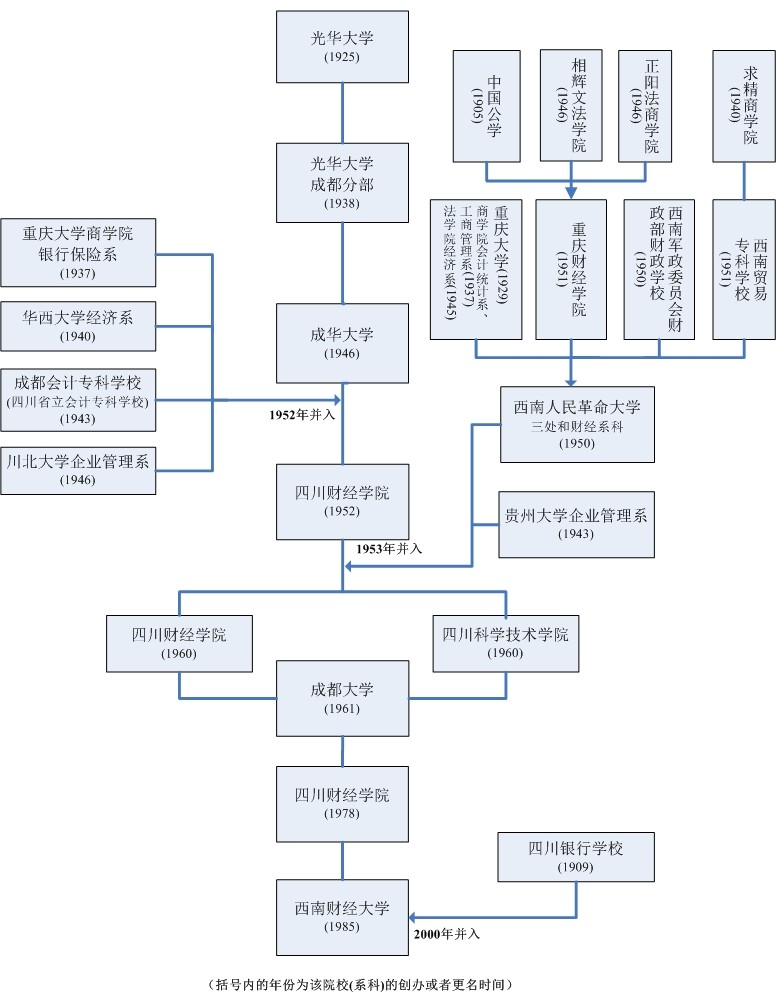
\includegraphics[width=0.6\linewidth]{img/西南财经大学历史沿革简表.jpg}
\caption{西南财经大学历史沿革简表}
\label{fig:西南财经大学历史沿革简表}
\end{figure}

1952至1953年全国院系调整中,以成华大学为基础先后并入西南地区16所财经院校或综合大学的财经系科,组建四川财经学院,是建国之初全国高等院校分区布局中的四所财经学院之一,由国家高教部主管。学校荟萃了我国著名经济学家陈豹隐、李孝同、彭迪先等一批著名教授。1952年10月由西南军政委员会(1953年3月改建为西南行政委员会)领导,1954年1月划归四川省政府领导,1954年12月由中央政府高等教育部直管,1958年7月改由四川省政府主管。1960年分设四川财经学院和四川科学技术学院,1961年合并更名为成都大学,文革期间历尽沧桑,1978年恢复为四川财经学院。1979年划归中国人民银行主管,1985年更名为西南财经大学。2000年以独立建制划转教育部管理。

1997年进入国家“211工程”建设高校,2010年成为国家教育体制改革试点高校,2011年进入国家“985工程”优势学科创新平台建设高校。